% --- NVIDIA Cosmos: World Foundation Models for Physical AI ---
\begin{frame}[t]{NVIDIA Cosmos: a platform of World Foundation Models}
  \begin{itemize}\itemsep0.30em
    \item \textbf{What it is:} an open platform of \textbf{World Foundation Models (WFMs)} ---
          large pre-trained generative models of physical dynamics --- aimed at
          \textbf{Physical AI}: robots, autonomous vehicles, and embodied agents.
    \item \textbf{Why it exists:} real-world data collection for robotics/AV is slow, costly,
          and unsafe. Cosmos generates \textbf{physically plausible, controllable video}
          to simulate, augment, and pre-train policies at scale.
    \item \textbf{Two model families:}
      \begin{itemize}\itemsep0.18em
        \item \textbf{Cosmos-Predict} (diffusion + autoregressive WFMs) --- future-frame /
              video prediction from text, image, or video prompts.
        \item \textbf{Cosmos-Transfer} --- multimodal control (e.g.\ segmentation, depth,
              edges, LiDAR) for \textbf{sim-to-real} and data augmentation.
      \end{itemize}
    \item Trained on millions of hours of driving and robotics video; released with
          \textbf{open weights} and a permissive licence for research and industry.
  \end{itemize}
\end{frame}

\begin{frame}[t]{Cosmos: pipeline, tokenizer, and where it fits}
  \begin{columns}[T,onlytextwidth]
    \begin{column}{0.56\textwidth}
      \textbf{Key components}
      \begin{itemize}\itemsep0.22em
        \item \textbf{Cosmos Tokenizer:} high-compression, high-fidelity visual tokenizer
              (continuous \emph{and} discrete) that makes long-video training tractable.
        \item \textbf{Curated data pipeline:} large-scale filtering, captioning, and dedup of
              physical-world video.
        \item \textbf{Post-training / guardrails:} adapt a base WFM to a downstream embodiment
              (e.g.\ a specific robot or camera rig); safety filters on inputs and outputs.
      \end{itemize}
    \end{column}
    \begin{column}{0.44\textwidth}
      \textbf{How it connects to this lecture}
      \begin{itemize}\itemsep0.22em
        \item A \textbf{generative} world model (like Sora/Genie), but explicitly engineered as
              \textbf{infrastructure} for Physical AI rather than media synthesis.
        \item Emphasises \textbf{controllability} and \textbf{action/condition grounding} ---
              the bridge from ``pretty video'' toward usable \textbf{simulators}.
        \item Reinforces the lecture's theme: the \textbf{simulation gap} is being closed
              with data, control signals, and scale.
      \end{itemize}
      \vspace{0.3em}
      {\footnotesize NVIDIA, ``Cosmos World Foundation Model Platform for Physical AI''
      (\href{https://arxiv.org/abs/2501.03575}{arXiv:2501.03575});
      \href{https://www.nvidia.com/en-us/ai/cosmos/}{nvidia.com/en-us/ai/cosmos};
      code: \href{https://github.com/NVIDIA/Cosmos}{github.com/NVIDIA/Cosmos}.}
    \end{column}
  \end{columns}
\end{frame}

\begin{frame}[t]{Cosmos: model architecture}
  \centering
  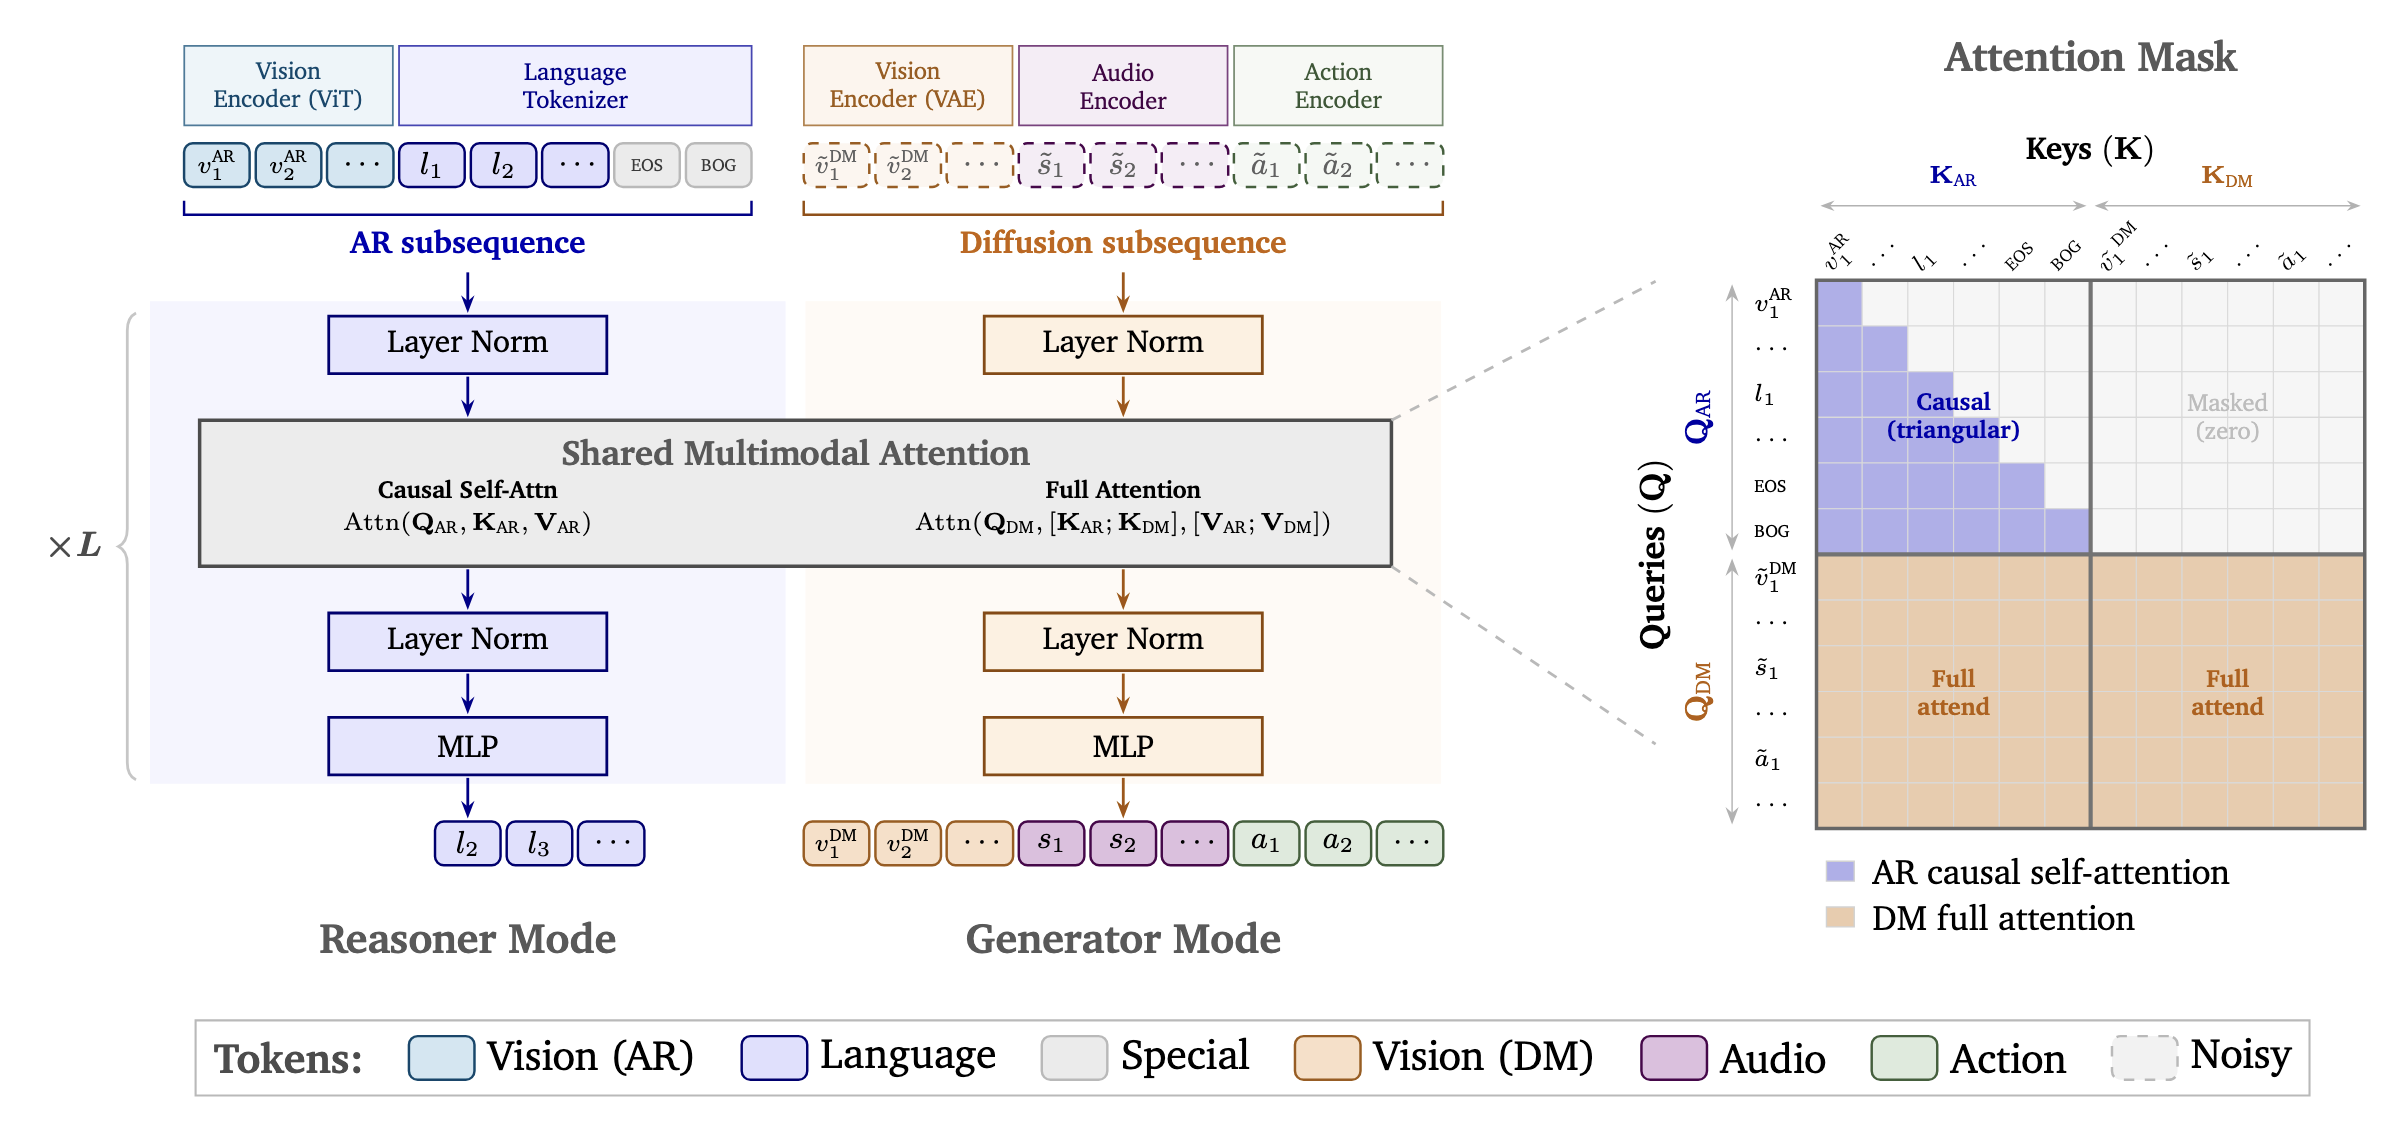
\includegraphics[width=\linewidth,height=0.82\textheight,keepaspectratio]{images/cosmos3/cosmos3-model-architecture.png}\\[0.28em]
  {\scriptsize Cosmos world-foundation-model architecture. Source: NVIDIA Cosmos
  (\href{https://github.com/NVIDIA/Cosmos}{github.com/NVIDIA/Cosmos}; \href{https://arxiv.org/abs/2501.03575}{arXiv:2501.03575}).}
\end{frame}
